\begin{figure}[h]
    \centering
    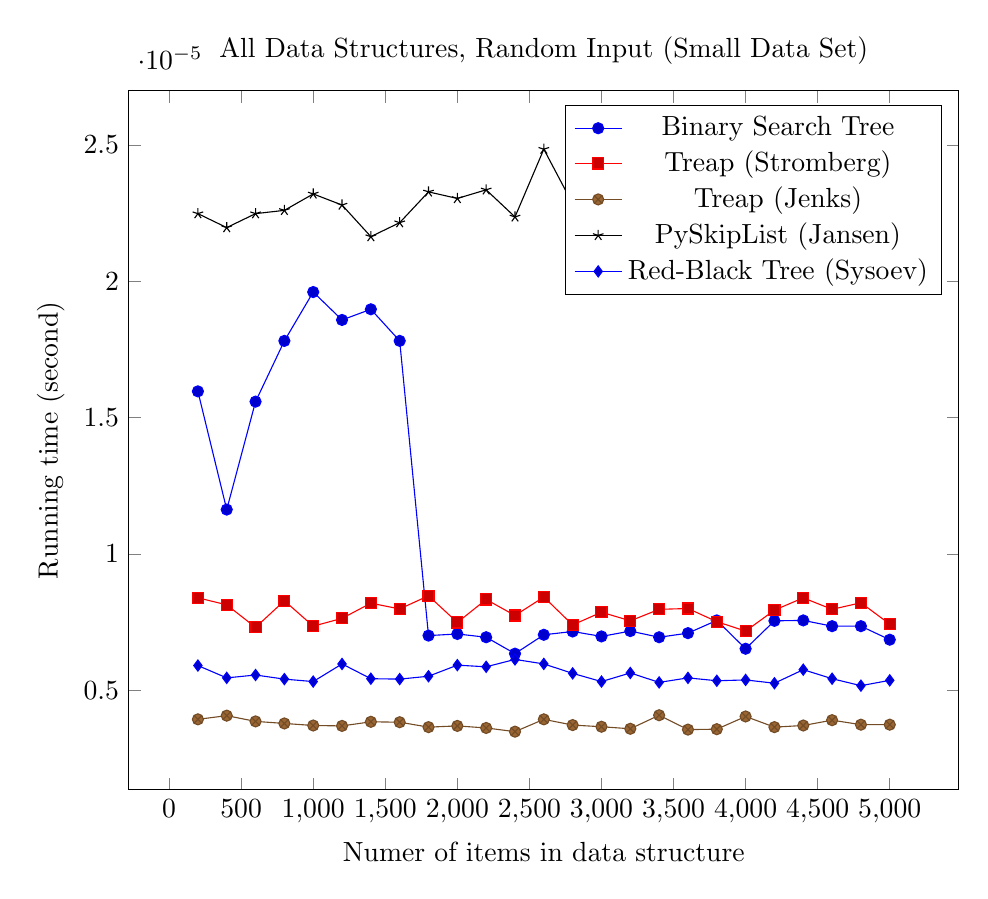
\begin{tikzpicture}
        \begin{axis}[
            xlabel={Numer of items in data structure},
            ylabel={Running time (second)},
            title={All Data Structures, Random Input (Small Data Set)},
            width=\textwidth
        ]
		\addplot coordinates {
			(200, 1.5962292847837567e-05)
			(400, 1.1625367998613356e-05)
			(600, 1.5585823676900202e-05)
			(800, 1.78145211688574e-05)
			(1000, 1.960651442253214e-05)
			(1200, 1.858251827757673e-05)
			(1400, 1.8974046215358697e-05)
			(1600, 1.78145211688574e-05)
			(1800, 7.002326579474971e-06)
			(2000, 7.062561646831167e-06)
			(2200, 6.942091512129878e-06)
			(2400, 6.339740838623431e-06)
			(2600, 7.032444113141967e-06)
			(2800, 7.152914247854358e-06)
			(3000, 6.972209045796873e-06)
			(3200, 7.167973014698958e-06)
			(3400, 6.942091512118776e-06)
			(3600, 7.092679180509265e-06)
			(3800, 7.559500952469822e-06)
			(4000, 6.520446040669814e-06)
			(4200, 7.544442185625222e-06)
			(4400, 7.5595009524587194e-06)
			(4600, 7.348678216745341e-06)
			(4800, 7.348678216745341e-06)
			(5000, 6.8517389111066865e-06)
		};
		\addplot coordinates {
			(200, 8.387733128534247e-06)
			(400, 8.131734092287069e-06)
			(600, 7.303501916222644e-06)
			(800, 8.282321760666455e-06)
			(1000, 7.348678216745341e-06)
			(1200, 7.634794786659516e-06)
			(1400, 8.191969159654366e-06)
			(1600, 7.981146423918783e-06)
			(1800, 8.46302696272394e-06)
			(2000, 7.484207118280128e-06)
			(2200, 8.327498061178051e-06)
			(2400, 7.740206154516205e-06)
			(2600, 8.417850662212345e-06)
			(2800, 7.393854517245835e-06)
			(3000, 7.860676289217494e-06)
			(3200, 7.544442185636324e-06)
			(3400, 7.966087657074183e-06)
			(3600, 7.996205190763384e-06)
			(3800, 7.514324651958226e-06)
			(4000, 7.167973014687856e-06)
			(4200, 7.935970123396086e-06)
			(4400, 8.387733128534247e-06)
			(4600, 7.966087657085286e-06)
			(4800, 8.207027926476762e-06)
			(5000, 7.423972050923933e-06)
		};
		\addplot coordinates {
			(200, 3.930338144608747e-06)
			(400, 4.0658670461546365e-06)
			(600, 3.855044310419054e-06)
			(800, 3.7797504762293597e-06)
			(1000, 3.7044566420507685e-06)
			(1200, 3.6893978752061685e-06)
			(1400, 3.839985543585556e-06)
			(1600, 3.824926776752058e-06)
			(1800, 3.644221574694573e-06)
			(2000, 3.6893978752061685e-06)
			(2200, 3.6141040410164748e-06)
			(2400, 3.478575139481688e-06)
			(2600, 3.930338144608747e-06)
			(2800, 3.7195154088842665e-06)
			(3000, 3.6592803415280704e-06)
			(3200, 3.583986507349479e-06)
			(3400, 4.0809258129881345e-06)
			(3600, 3.553868973671381e-06)
			(3800, 3.5689277405159812e-06)
			(4000, 4.035749512476538e-06)
			(4200, 3.644221574694573e-06)
			(4400, 3.7044566420507685e-06)
			(4600, 3.900220610941751e-06)
			(4800, 3.7345741757288666e-06)
			(5000, 3.734574175717764e-06)
		};
		\addplot coordinates {
			(200, 2.248273888850738e-05)
			(400, 2.1970740816035227e-05)
			(600, 2.248273888850738e-05)
			(800, 2.260320902320867e-05)
			(1000, 2.3205559696715117e-05)
			(1200, 2.2798972992099652e-05)
			(1400, 2.163944794560946e-05)
			(1600, 2.215144601808161e-05)
			(1800, 2.328085353090481e-05)
			(2000, 2.303991326150223e-05)
			(2200, 2.3356147365094504e-05)
			(2400, 2.2362268753806092e-05)
			(2600, 2.484696528201047e-05)
			(2800, 2.2844149292622352e-05)
			(3000, 2.3672381468675675e-05)
			(3200, 2.22869749196275e-05)
			(3400, 2.2347209986972595e-05)
			(3600, 2.3582028867652483e-05)
			(3800, 2.2106269717570016e-05)
			(4000, 2.3235677230393215e-05)
			(4200, 2.328085353090481e-05)
			(4400, 2.3024854494668733e-05)
			(4600, 2.1684624246121054e-05)
			(4800, 2.3536852567140888e-05)
			(5000, 2.459096624577439e-05)
		};
		\addplot coordinates {
			(200, 5.903036600329869e-06)
			(400, 5.45127359520281e-06)
			(600, 5.556684963059499e-06)
			(800, 5.406097294691215e-06)
			(1000, 5.315744693668023e-06)
			(1200, 5.963271667674963e-06)
			(1400, 5.421156061535815e-06)
			(1600, 5.406097294691215e-06)
			(1800, 5.511508662547904e-06)
			(2000, 5.918095367163367e-06)
			(2200, 5.857860299818274e-06)
			(2400, 6.128918102898951e-06)
			(2600, 5.963271667674963e-06)
			(2800, 5.616920030415695e-06)
			(3000, 5.315744693656921e-06)
			(3200, 5.631978797249193e-06)
			(3400, 5.2856271599899255e-06)
			(3600, 5.45127359520281e-06)
			(3800, 5.345862227335019e-06)
			(4000, 5.375979761013117e-06)
			(4200, 5.2555096263118274e-06)
			(4400, 5.752448931961585e-06)
			(4600, 5.421156061535815e-06)
			(4800, 5.165157025288636e-06)
			(5000, 5.360920994179619e-06)
		};
        \legend{Binary Search Tree, Treap (Stromberg), Treap (Jenks), PySkipList (Jansen), Red-Black Tree (Sysoev)}
        \end{axis}
    \end{tikzpicture}
    \caption{Average of 20 operations, benchmarked every 200, starting at 200.}
\end{figure}